\documentclass[11pt]{article}

    \usepackage[breakable]{tcolorbox}
    \usepackage{parskip} % Stop auto-indenting (to mimic markdown behaviour)
    

    % Basic figure setup, for now with no caption control since it's done
    % automatically by Pandoc (which extracts ![](path) syntax from Markdown).
    \usepackage{graphicx}
    % Maintain compatibility with old templates. Remove in nbconvert 6.0
    \let\Oldincludegraphics\includegraphics
    % Ensure that by default, figures have no caption (until we provide a
    % proper Figure object with a Caption API and a way to capture that
    % in the conversion process - todo).
    \usepackage{caption}
    %\DeclareCaptionFormat{nocaption}{}
    %\captionsetup{format=nocaption,aboveskip=0pt,belowskip=0pt}

    \usepackage{float}
    \floatplacement{figure}{H} % forces figures to be placed at the correct location
    \usepackage{xcolor} % Allow colors to be defined
    \usepackage{enumerate} % Needed for markdown enumerations to work
    \usepackage{geometry} % Used to adjust the document margins
    \usepackage{amsmath} % Equations
    \usepackage{amssymb} % Equations
    \usepackage{textcomp} % defines textquotesingle
    % Hack from http://tex.stackexchange.com/a/47451/13684:
    \AtBeginDocument{%
        \def\PYZsq{\textquotesingle}% Upright quotes in Pygmentized code
    }
    \usepackage{upquote} % Upright quotes for verbatim code
    \usepackage{eurosym} % defines \euro

    \usepackage{iftex}
    \ifPDFTeX
        \usepackage[T1]{fontenc}
        \IfFileExists{alphabeta.sty}{
              \usepackage{alphabeta}
          }{
              \usepackage[mathletters]{ucs}
              \usepackage[utf8x]{inputenc}
          }
    \else
        \usepackage{fontspec}
        \usepackage{unicode-math}
    \fi

    \usepackage{fancyvrb} % verbatim replacement that allows latex
    \usepackage{grffile} % extends the file name processing of package graphics 
                         % to support a larger range
    \makeatletter % fix for old versions of grffile with XeLaTeX
    \@ifpackagelater{grffile}{2019/11/01}
    {
      % Do nothing on new versions
    }
    {
      \def\Gread@@xetex#1{%
        \IfFileExists{"\Gin@base".bb}%
        {\Gread@eps{\Gin@base.bb}}%
        {\Gread@@xetex@aux#1}%
      }
    }
    \makeatother
    \usepackage[Export]{adjustbox} % Used to constrain images to a maximum size
    \adjustboxset{max size={0.9\linewidth}{0.9\paperheight}}

    % The hyperref package gives us a pdf with properly built
    % internal navigation ('pdf bookmarks' for the table of contents,
    % internal cross-reference links, web links for URLs, etc.)
    \usepackage{hyperref}
    % The default LaTeX title has an obnoxious amount of whitespace. By default,
    % titling removes some of it. It also provides customization options.
    \usepackage{titling}
    \usepackage{longtable} % longtable support required by pandoc >1.10
    \usepackage{booktabs}  % table support for pandoc > 1.12.2
    \usepackage{array}     % table support for pandoc >= 2.11.3
    \usepackage{calc}      % table minipage width calculation for pandoc >= 2.11.1
    \usepackage[inline]{enumitem} % IRkernel/repr support (it uses the enumerate* environment)
    \usepackage[normalem]{ulem} % ulem is needed to support strikethroughs (\sout)
                                % normalem makes italics be italics, not underlines
    \usepackage{mathrsfs}
    \usepackage{listings}
    \usepackage{xcolor}

\definecolor{codegreen}{rgb}{0,0.6,0}
\definecolor{codegray}{rgb}{0.5,0.5,0.5}
\definecolor{codepurple}{rgb}{0.58,0,0.82}
\definecolor{backcolour}{rgb}{0.95,0.95,0.92}

\lstdefinestyle{mystyle}{
    backgroundcolor=\color{backcolour},   
    commentstyle=\color{codegreen},
    keywordstyle=\color{magenta},
    numberstyle=\tiny\color{codegray},
    stringstyle=\color{codepurple},
    basicstyle=\ttfamily\footnotesize,
    breakatwhitespace=false,         
    breaklines=true,                 
    captionpos=b,                    
    keepspaces=true,                 
    numbers=left,                    
    numbersep=5pt,                  
    showspaces=false,                
    showstringspaces=false,
    showtabs=false,                  
    tabsize=2
}

\lstset{style=mystyle}
    

    
    % Colors for the hyperref package
    \definecolor{urlcolor}{rgb}{0,.145,.698}
    \definecolor{linkcolor}{rgb}{0,.145,.698}
    \definecolor{citecolor}{rgb}{.12,.54,.11}

    % ANSI colors
    \definecolor{ansi-black}{HTML}{3E424D}
    \definecolor{ansi-black-intense}{HTML}{282C36}
    \definecolor{ansi-red}{HTML}{E75C58}
    \definecolor{ansi-red-intense}{HTML}{B22B31}
    \definecolor{ansi-green}{HTML}{00A250}
    \definecolor{ansi-green-intense}{HTML}{007427}
    \definecolor{ansi-yellow}{HTML}{DDB62B}
    \definecolor{ansi-yellow-intense}{HTML}{B27D12}
    \definecolor{ansi-blue}{HTML}{208FFB}
    \definecolor{ansi-blue-intense}{HTML}{0065CA}
    \definecolor{ansi-magenta}{HTML}{D160C4}
    \definecolor{ansi-magenta-intense}{HTML}{A03196}
    \definecolor{ansi-cyan}{HTML}{60C6C8}
    \definecolor{ansi-cyan-intense}{HTML}{258F8F}
    \definecolor{ansi-white}{HTML}{C5C1B4}
    \definecolor{ansi-white-intense}{HTML}{A1A6B2}
    \definecolor{ansi-default-inverse-fg}{HTML}{FFFFFF}
    \definecolor{ansi-default-inverse-bg}{HTML}{000000}

    % common color for the border for error outputs.
    \definecolor{outerrorbackground}{HTML}{FFDFDF}

    % commands and environments needed by pandoc snippets
    % extracted from the output of `pandoc -s`
    \providecommand{\tightlist}{%
      \setlength{\itemsep}{0pt}\setlength{\parskip}{0pt}}
    \DefineVerbatimEnvironment{Highlighting}{Verbatim}{commandchars=\\\{\}}
    % Add ',fontsize=\small' for more characters per line
    \newenvironment{Shaded}{}{}
    \newcommand{\KeywordTok}[1]{\textcolor[rgb]{0.00,0.44,0.13}{\textbf{{#1}}}}
    \newcommand{\DataTypeTok}[1]{\textcolor[rgb]{0.56,0.13,0.00}{{#1}}}
    \newcommand{\DecValTok}[1]{\textcolor[rgb]{0.25,0.63,0.44}{{#1}}}
    \newcommand{\BaseNTok}[1]{\textcolor[rgb]{0.25,0.63,0.44}{{#1}}}
    \newcommand{\FloatTok}[1]{\textcolor[rgb]{0.25,0.63,0.44}{{#1}}}
    \newcommand{\CharTok}[1]{\textcolor[rgb]{0.25,0.44,0.63}{{#1}}}
    \newcommand{\StringTok}[1]{\textcolor[rgb]{0.25,0.44,0.63}{{#1}}}
    \newcommand{\CommentTok}[1]{\textcolor[rgb]{0.38,0.63,0.69}{\textit{{#1}}}}
    \newcommand{\OtherTok}[1]{\textcolor[rgb]{0.00,0.44,0.13}{{#1}}}
    \newcommand{\AlertTok}[1]{\textcolor[rgb]{1.00,0.00,0.00}{\textbf{{#1}}}}
    \newcommand{\FunctionTok}[1]{\textcolor[rgb]{0.02,0.16,0.49}{{#1}}}
    \newcommand{\RegionMarkerTok}[1]{{#1}}
    \newcommand{\ErrorTok}[1]{\textcolor[rgb]{1.00,0.00,0.00}{\textbf{{#1}}}}
    \newcommand{\NormalTok}[1]{{#1}}
    
    % Additional commands for more recent versions of Pandoc
    \newcommand{\ConstantTok}[1]{\textcolor[rgb]{0.53,0.00,0.00}{{#1}}}
    \newcommand{\SpecialCharTok}[1]{\textcolor[rgb]{0.25,0.44,0.63}{{#1}}}
    \newcommand{\VerbatimStringTok}[1]{\textcolor[rgb]{0.25,0.44,0.63}{{#1}}}
    \newcommand{\SpecialStringTok}[1]{\textcolor[rgb]{0.73,0.40,0.53}{{#1}}}
    \newcommand{\ImportTok}[1]{{#1}}
    \newcommand{\DocumentationTok}[1]{\textcolor[rgb]{0.73,0.13,0.13}{\textit{{#1}}}}
    \newcommand{\AnnotationTok}[1]{\textcolor[rgb]{0.38,0.63,0.69}{\textbf{\textit{{#1}}}}}
    \newcommand{\CommentVarTok}[1]{\textcolor[rgb]{0.38,0.63,0.69}{\textbf{\textit{{#1}}}}}
    \newcommand{\VariableTok}[1]{\textcolor[rgb]{0.10,0.09,0.49}{{#1}}}
    \newcommand{\ControlFlowTok}[1]{\textcolor[rgb]{0.00,0.44,0.13}{\textbf{{#1}}}}
    \newcommand{\OperatorTok}[1]{\textcolor[rgb]{0.40,0.40,0.40}{{#1}}}
    \newcommand{\BuiltInTok}[1]{{#1}}
    \newcommand{\ExtensionTok}[1]{{#1}}
    \newcommand{\PreprocessorTok}[1]{\textcolor[rgb]{0.74,0.48,0.00}{{#1}}}
    \newcommand{\AttributeTok}[1]{\textcolor[rgb]{0.49,0.56,0.16}{{#1}}}
    \newcommand{\InformationTok}[1]{\textcolor[rgb]{0.38,0.63,0.69}{\textbf{\textit{{#1}}}}}
    \newcommand{\WarningTok}[1]{\textcolor[rgb]{0.38,0.63,0.69}{\textbf{\textit{{#1}}}}}
    
    
    % Define a nice break command that doesn't care if a line doesn't already
    % exist.
    \def\br{\hspace*{\fill} \\* }
    % Math Jax compatibility definitions
    \def\gt{>}
    \def\lt{<}
    \let\Oldtex\TeX
    \let\Oldlatex\LaTeX
    \renewcommand{\TeX}{\textrm{\Oldtex}}
    \renewcommand{\LaTeX}{\textrm{\Oldlatex}}
    % Document parameters
    % Document title
    \title{PEC 1}
    
    
    
    
    
% Pygments definitions
\makeatletter
\def\PY@reset{\let\PY@it=\relax \let\PY@bf=\relax%
    \let\PY@ul=\relax \let\PY@tc=\relax%
    \let\PY@bc=\relax \let\PY@ff=\relax}
\def\PY@tok#1{\csname PY@tok@#1\endcsname}
\def\PY@toks#1+{\ifx\relax#1\empty\else%
    \PY@tok{#1}\expandafter\PY@toks\fi}
\def\PY@do#1{\PY@bc{\PY@tc{\PY@ul{%
    \PY@it{\PY@bf{\PY@ff{#1}}}}}}}
\def\PY#1#2{\PY@reset\PY@toks#1+\relax+\PY@do{#2}}

\@namedef{PY@tok@w}{\def\PY@tc##1{\textcolor[rgb]{0.73,0.73,0.73}{##1}}}
\@namedef{PY@tok@c}{\let\PY@it=\textit\def\PY@tc##1{\textcolor[rgb]{0.24,0.48,0.48}{##1}}}
\@namedef{PY@tok@cp}{\def\PY@tc##1{\textcolor[rgb]{0.61,0.40,0.00}{##1}}}
\@namedef{PY@tok@k}{\let\PY@bf=\textbf\def\PY@tc##1{\textcolor[rgb]{0.00,0.50,0.00}{##1}}}
\@namedef{PY@tok@kp}{\def\PY@tc##1{\textcolor[rgb]{0.00,0.50,0.00}{##1}}}
\@namedef{PY@tok@kt}{\def\PY@tc##1{\textcolor[rgb]{0.69,0.00,0.25}{##1}}}
\@namedef{PY@tok@o}{\def\PY@tc##1{\textcolor[rgb]{0.40,0.40,0.40}{##1}}}
\@namedef{PY@tok@ow}{\let\PY@bf=\textbf\def\PY@tc##1{\textcolor[rgb]{0.67,0.13,1.00}{##1}}}
\@namedef{PY@tok@nb}{\def\PY@tc##1{\textcolor[rgb]{0.00,0.50,0.00}{##1}}}
\@namedef{PY@tok@nf}{\def\PY@tc##1{\textcolor[rgb]{0.00,0.00,1.00}{##1}}}
\@namedef{PY@tok@nc}{\let\PY@bf=\textbf\def\PY@tc##1{\textcolor[rgb]{0.00,0.00,1.00}{##1}}}
\@namedef{PY@tok@nn}{\let\PY@bf=\textbf\def\PY@tc##1{\textcolor[rgb]{0.00,0.00,1.00}{##1}}}
\@namedef{PY@tok@ne}{\let\PY@bf=\textbf\def\PY@tc##1{\textcolor[rgb]{0.80,0.25,0.22}{##1}}}
\@namedef{PY@tok@nv}{\def\PY@tc##1{\textcolor[rgb]{0.10,0.09,0.49}{##1}}}
\@namedef{PY@tok@no}{\def\PY@tc##1{\textcolor[rgb]{0.53,0.00,0.00}{##1}}}
\@namedef{PY@tok@nl}{\def\PY@tc##1{\textcolor[rgb]{0.46,0.46,0.00}{##1}}}
\@namedef{PY@tok@ni}{\let\PY@bf=\textbf\def\PY@tc##1{\textcolor[rgb]{0.44,0.44,0.44}{##1}}}
\@namedef{PY@tok@na}{\def\PY@tc##1{\textcolor[rgb]{0.41,0.47,0.13}{##1}}}
\@namedef{PY@tok@nt}{\let\PY@bf=\textbf\def\PY@tc##1{\textcolor[rgb]{0.00,0.50,0.00}{##1}}}
\@namedef{PY@tok@nd}{\def\PY@tc##1{\textcolor[rgb]{0.67,0.13,1.00}{##1}}}
\@namedef{PY@tok@s}{\def\PY@tc##1{\textcolor[rgb]{0.73,0.13,0.13}{##1}}}
\@namedef{PY@tok@sd}{\let\PY@it=\textit\def\PY@tc##1{\textcolor[rgb]{0.73,0.13,0.13}{##1}}}
\@namedef{PY@tok@si}{\let\PY@bf=\textbf\def\PY@tc##1{\textcolor[rgb]{0.64,0.35,0.47}{##1}}}
\@namedef{PY@tok@se}{\let\PY@bf=\textbf\def\PY@tc##1{\textcolor[rgb]{0.67,0.36,0.12}{##1}}}
\@namedef{PY@tok@sr}{\def\PY@tc##1{\textcolor[rgb]{0.64,0.35,0.47}{##1}}}
\@namedef{PY@tok@ss}{\def\PY@tc##1{\textcolor[rgb]{0.10,0.09,0.49}{##1}}}
\@namedef{PY@tok@sx}{\def\PY@tc##1{\textcolor[rgb]{0.00,0.50,0.00}{##1}}}
\@namedef{PY@tok@m}{\def\PY@tc##1{\textcolor[rgb]{0.40,0.40,0.40}{##1}}}
\@namedef{PY@tok@gh}{\let\PY@bf=\textbf\def\PY@tc##1{\textcolor[rgb]{0.00,0.00,0.50}{##1}}}
\@namedef{PY@tok@gu}{\let\PY@bf=\textbf\def\PY@tc##1{\textcolor[rgb]{0.50,0.00,0.50}{##1}}}
\@namedef{PY@tok@gd}{\def\PY@tc##1{\textcolor[rgb]{0.63,0.00,0.00}{##1}}}
\@namedef{PY@tok@gi}{\def\PY@tc##1{\textcolor[rgb]{0.00,0.52,0.00}{##1}}}
\@namedef{PY@tok@gr}{\def\PY@tc##1{\textcolor[rgb]{0.89,0.00,0.00}{##1}}}
\@namedef{PY@tok@ge}{\let\PY@it=\textit}
\@namedef{PY@tok@gs}{\let\PY@bf=\textbf}
\@namedef{PY@tok@gp}{\let\PY@bf=\textbf\def\PY@tc##1{\textcolor[rgb]{0.00,0.00,0.50}{##1}}}
\@namedef{PY@tok@go}{\def\PY@tc##1{\textcolor[rgb]{0.44,0.44,0.44}{##1}}}
\@namedef{PY@tok@gt}{\def\PY@tc##1{\textcolor[rgb]{0.00,0.27,0.87}{##1}}}
\@namedef{PY@tok@err}{\def\PY@bc##1{{\setlength{\fboxsep}{\string -\fboxrule}\fcolorbox[rgb]{1.00,0.00,0.00}{1,1,1}{\strut ##1}}}}
\@namedef{PY@tok@kc}{\let\PY@bf=\textbf\def\PY@tc##1{\textcolor[rgb]{0.00,0.50,0.00}{##1}}}
\@namedef{PY@tok@kd}{\let\PY@bf=\textbf\def\PY@tc##1{\textcolor[rgb]{0.00,0.50,0.00}{##1}}}
\@namedef{PY@tok@kn}{\let\PY@bf=\textbf\def\PY@tc##1{\textcolor[rgb]{0.00,0.50,0.00}{##1}}}
\@namedef{PY@tok@kr}{\let\PY@bf=\textbf\def\PY@tc##1{\textcolor[rgb]{0.00,0.50,0.00}{##1}}}
\@namedef{PY@tok@bp}{\def\PY@tc##1{\textcolor[rgb]{0.00,0.50,0.00}{##1}}}
\@namedef{PY@tok@fm}{\def\PY@tc##1{\textcolor[rgb]{0.00,0.00,1.00}{##1}}}
\@namedef{PY@tok@vc}{\def\PY@tc##1{\textcolor[rgb]{0.10,0.09,0.49}{##1}}}
\@namedef{PY@tok@vg}{\def\PY@tc##1{\textcolor[rgb]{0.10,0.09,0.49}{##1}}}
\@namedef{PY@tok@vi}{\def\PY@tc##1{\textcolor[rgb]{0.10,0.09,0.49}{##1}}}
\@namedef{PY@tok@vm}{\def\PY@tc##1{\textcolor[rgb]{0.10,0.09,0.49}{##1}}}
\@namedef{PY@tok@sa}{\def\PY@tc##1{\textcolor[rgb]{0.73,0.13,0.13}{##1}}}
\@namedef{PY@tok@sb}{\def\PY@tc##1{\textcolor[rgb]{0.73,0.13,0.13}{##1}}}
\@namedef{PY@tok@sc}{\def\PY@tc##1{\textcolor[rgb]{0.73,0.13,0.13}{##1}}}
\@namedef{PY@tok@dl}{\def\PY@tc##1{\textcolor[rgb]{0.73,0.13,0.13}{##1}}}
\@namedef{PY@tok@s2}{\def\PY@tc##1{\textcolor[rgb]{0.73,0.13,0.13}{##1}}}
\@namedef{PY@tok@sh}{\def\PY@tc##1{\textcolor[rgb]{0.73,0.13,0.13}{##1}}}
\@namedef{PY@tok@s1}{\def\PY@tc##1{\textcolor[rgb]{0.73,0.13,0.13}{##1}}}
\@namedef{PY@tok@mb}{\def\PY@tc##1{\textcolor[rgb]{0.40,0.40,0.40}{##1}}}
\@namedef{PY@tok@mf}{\def\PY@tc##1{\textcolor[rgb]{0.40,0.40,0.40}{##1}}}
\@namedef{PY@tok@mh}{\def\PY@tc##1{\textcolor[rgb]{0.40,0.40,0.40}{##1}}}
\@namedef{PY@tok@mi}{\def\PY@tc##1{\textcolor[rgb]{0.40,0.40,0.40}{##1}}}
\@namedef{PY@tok@il}{\def\PY@tc##1{\textcolor[rgb]{0.40,0.40,0.40}{##1}}}
\@namedef{PY@tok@mo}{\def\PY@tc##1{\textcolor[rgb]{0.40,0.40,0.40}{##1}}}
\@namedef{PY@tok@ch}{\let\PY@it=\textit\def\PY@tc##1{\textcolor[rgb]{0.24,0.48,0.48}{##1}}}
\@namedef{PY@tok@cm}{\let\PY@it=\textit\def\PY@tc##1{\textcolor[rgb]{0.24,0.48,0.48}{##1}}}
\@namedef{PY@tok@cpf}{\let\PY@it=\textit\def\PY@tc##1{\textcolor[rgb]{0.24,0.48,0.48}{##1}}}
\@namedef{PY@tok@c1}{\let\PY@it=\textit\def\PY@tc##1{\textcolor[rgb]{0.24,0.48,0.48}{##1}}}
\@namedef{PY@tok@cs}{\let\PY@it=\textit\def\PY@tc##1{\textcolor[rgb]{0.24,0.48,0.48}{##1}}}

\def\PYZbs{\char`\\}
\def\PYZus{\char`\_}
\def\PYZob{\char`\{}
\def\PYZcb{\char`\}}
\def\PYZca{\char`\^}
\def\PYZam{\char`\&}
\def\PYZlt{\char`\<}
\def\PYZgt{\char`\>}
\def\PYZsh{\char`\#}
\def\PYZpc{\char`\%}
\def\PYZdl{\char`\$}
\def\PYZhy{\char`\-}
\def\PYZsq{\char`\'}
\def\PYZdq{\char`\"}
\def\PYZti{\char`\~}
% for compatibility with earlier versions
\def\PYZat{@}
\def\PYZlb{[}
\def\PYZrb{]}
\makeatother


    % For linebreaks inside Verbatim environment from package fancyvrb. 
    \makeatletter
        \newbox\Wrappedcontinuationbox 
        \newbox\Wrappedvisiblespacebox 
        \newcommand*\Wrappedvisiblespace {\textcolor{red}{\textvisiblespace}} 
        \newcommand*\Wrappedcontinuationsymbol {\textcolor{red}{\llap{\tiny$\m@th\hookrightarrow$}}} 
        \newcommand*\Wrappedcontinuationindent {3ex } 
        \newcommand*\Wrappedafterbreak {\kern\Wrappedcontinuationindent\copy\Wrappedcontinuationbox} 
        % Take advantage of the already applied Pygments mark-up to insert 
        % potential linebreaks for TeX processing. 
        %        {, <, #, %, $, ' and ": go to next line. 
        %        _, }, ^, &, >, - and ~: stay at end of broken line. 
        % Use of \textquotesingle for straight quote. 
        \newcommand*\Wrappedbreaksatspecials {% 
            \def\PYGZus{\discretionary{\char`\_}{\Wrappedafterbreak}{\char`\_}}% 
            \def\PYGZob{\discretionary{}{\Wrappedafterbreak\char`\{}{\char`\{}}% 
            \def\PYGZcb{\discretionary{\char`\}}{\Wrappedafterbreak}{\char`\}}}% 
            \def\PYGZca{\discretionary{\char`\^}{\Wrappedafterbreak}{\char`\^}}% 
            \def\PYGZam{\discretionary{\char`\&}{\Wrappedafterbreak}{\char`\&}}% 
            \def\PYGZlt{\discretionary{}{\Wrappedafterbreak\char`\<}{\char`\<}}% 
            \def\PYGZgt{\discretionary{\char`\>}{\Wrappedafterbreak}{\char`\>}}% 
            \def\PYGZsh{\discretionary{}{\Wrappedafterbreak\char`\#}{\char`\#}}% 
            \def\PYGZpc{\discretionary{}{\Wrappedafterbreak\char`\%}{\char`\%}}% 
            \def\PYGZdl{\discretionary{}{\Wrappedafterbreak\char`\$}{\char`\$}}% 
            \def\PYGZhy{\discretionary{\char`\-}{\Wrappedafterbreak}{\char`\-}}% 
            \def\PYGZsq{\discretionary{}{\Wrappedafterbreak\textquotesingle}{\textquotesingle}}% 
            \def\PYGZdq{\discretionary{}{\Wrappedafterbreak\char`\"}{\char`\"}}% 
            \def\PYGZti{\discretionary{\char`\~}{\Wrappedafterbreak}{\char`\~}}% 
        } 
        % Some characters . , ; ? ! / are not pygmentized. 
        % This macro makes them "active" and they will insert potential linebreaks 
        \newcommand*\Wrappedbreaksatpunct {% 
            \lccode`\~`\.\lowercase{\def~}{\discretionary{\hbox{\char`\.}}{\Wrappedafterbreak}{\hbox{\char`\.}}}% 
            \lccode`\~`\,\lowercase{\def~}{\discretionary{\hbox{\char`\,}}{\Wrappedafterbreak}{\hbox{\char`\,}}}% 
            \lccode`\~`\;\lowercase{\def~}{\discretionary{\hbox{\char`\;}}{\Wrappedafterbreak}{\hbox{\char`\;}}}% 
            \lccode`\~`\:\lowercase{\def~}{\discretionary{\hbox{\char`\:}}{\Wrappedafterbreak}{\hbox{\char`\:}}}% 
            \lccode`\~`\?\lowercase{\def~}{\discretionary{\hbox{\char`\?}}{\Wrappedafterbreak}{\hbox{\char`\?}}}% 
            \lccode`\~`\!\lowercase{\def~}{\discretionary{\hbox{\char`\!}}{\Wrappedafterbreak}{\hbox{\char`\!}}}% 
            \lccode`\~`\/\lowercase{\def~}{\discretionary{\hbox{\char`\/}}{\Wrappedafterbreak}{\hbox{\char`\/}}}% 
            \catcode`\.\active
            \catcode`\,\active 
            \catcode`\;\active
            \catcode`\:\active
            \catcode`\?\active
            \catcode`\!\active
            \catcode`\/\active 
            \lccode`\~`\~ 	
        }
    \makeatother

    \let\OriginalVerbatim=\Verbatim
    \makeatletter
    \renewcommand{\Verbatim}[1][1]{%
        %\parskip\z@skip
        \sbox\Wrappedcontinuationbox {\Wrappedcontinuationsymbol}%
        \sbox\Wrappedvisiblespacebox {\FV@SetupFont\Wrappedvisiblespace}%
        \def\FancyVerbFormatLine ##1{\hsize\linewidth
            \vtop{\raggedright\hyphenpenalty\z@\exhyphenpenalty\z@
                \doublehyphendemerits\z@\finalhyphendemerits\z@
                \strut ##1\strut}%
        }%
        % If the linebreak is at a space, the latter will be displayed as visible
        % space at end of first line, and a continuation symbol starts next line.
        % Stretch/shrink are however usually zero for typewriter font.
        \def\FV@Space {%
            \nobreak\hskip\z@ plus\fontdimen3\font minus\fontdimen4\font
            \discretionary{\copy\Wrappedvisiblespacebox}{\Wrappedafterbreak}
            {\kern\fontdimen2\font}%
        }%
        
        % Allow breaks at special characters using \PYG... macros.
        \Wrappedbreaksatspecials
        % Breaks at punctuation characters . , ; ? ! and / need catcode=\active 	
        \OriginalVerbatim[#1,codes*=\Wrappedbreaksatpunct]%
    }
    \makeatother

    % Exact colors from NB
    \definecolor{incolor}{HTML}{303F9F}
    \definecolor{outcolor}{HTML}{D84315}
    \definecolor{cellborder}{HTML}{CFCFCF}
    \definecolor{cellbackground}{HTML}{F7F7F7}
    
    % prompt
    \makeatletter
    \newcommand{\boxspacing}{\kern\kvtcb@left@rule\kern\kvtcb@boxsep}
    \makeatother
    \newcommand{\prompt}[4]{
        {\ttfamily\llap{{\color{#2}[#3]:\hspace{3pt}#4}}\vspace{-\baselineskip}}
    }
    

    
    % Prevent overflowing lines due to hard-to-break entities
    \sloppy 
    % Setup hyperref package
    \hypersetup{
      breaklinks=true,  % so long urls are correctly broken across lines
      colorlinks=true,
      urlcolor=urlcolor,
      linkcolor=linkcolor,
      citecolor=citecolor,
      }
    % Slightly bigger margins than the latex defaults
    
    \geometry{verbose,tmargin=1in,bmargin=1in,lmargin=1in,rmargin=1in}
    
    

\begin{document}
    \author{Pablo Riutort Grande}
    \maketitle
  
    
M0.538 - HIGH PERFORMANCE COMPUTING

MU Ingeniería Informática / MU Ingeniería Computacional y Matemática

Estudios de Informática, Multimedia y Telecomunicación

    \tableofcontents

       \newpage
\hypertarget{1}{%
\section{Performance evaluation: Sample parametric study}\label{1}}

\hypertarget{11}{%
\subsection{Provide the SGE script(s) and the shell scripts (or methodology, e.g.,
program, command sequence) that you used to carry out the parametric study's executions
systematically. Describe your choices (e.g., number of jobs launched vs. combinations in each
job).}\label{11}}

To do this exercise, 5 SGE scripts were developed, one for each call to app with different input parameters (10, 100, 500, 1000, 1500).

\begin{figure}[h]
\caption{Contents of HPC's home/PEC1 folder}
\centering
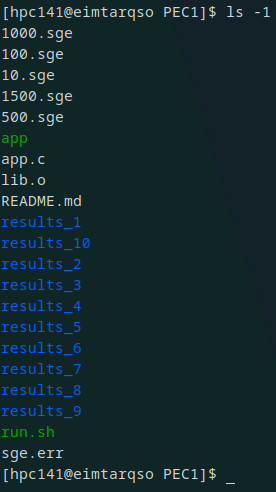
\includegraphics[width=0.5\textwidth]{ls.png}
\end{figure}

Each SGE script contains the following parameters:

\begin{itemize}
    \item \textbf{\#\$ -cwd}: Directs SGE to run the job in the same directory from which you submitted it.
    \item \textbf{\#\$ -S /bin/bash}: Specifies the interpreting shell for the job. 
    \item \textbf{\#\$ -N job\_name}: Sets the name of the job, in our case is specified with leading underscore followed by the input parameter (\_<number>).
    \item \textbf{\#\$ -o /dev/null}: Redirect standard output to null in order to avoid printing.
    \item \textbf{\#\$ -e sge.err}: Redirect error output to sge.err file
\end{itemize}

At the end of the SGE script we will find the command to run, each command will call the time command (not bash's) followed by a call to app with a given number. The time command will have the next parameters:

\begin{itemize}
    \item \textbf{-f \%e}: According to "time" manual, \%e will give "Elapsed real time (in seconds)"
    \item \textbf{-o results/<number>.txt}: Specifies the output file. One file per each input parameter in app.
\end{itemize}

\begin{lstlisting}[language=bash, caption=Contents of 10.sge script]
#!/bin/bash
#$ -cwd
#$ -S /bin/bash
#$ -N _10
#$ -o /dev/null
#$ -e sge.err

/usr/bin/time -f %e -o results/10.txt ./app 10

\end{lstlisting}

A run script helper was developed that calls each SGE script. For every call to this script a renaming of the directory results is needed in order to not let the next execution overwrite results, hence, we have results\_1, results\_2, and so on for every execution of the run script, 10 in total.

\begin{figure}[h]
\caption{Contents of results in fifth execution and 1000.txt file}
\centering
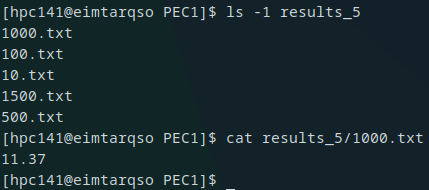
\includegraphics[width=0.5\textwidth]{results.png}
\end{figure}

\begin{lstlisting}[language=bash, caption=Contents of run.sh script]
#!/bin/sh

mkdir results
for j in 10 100 500 1000 1500
do
	qsub "$j.sge"
done
watch -n 2 -d qstat

\end{lstlisting}

run.sh will iterate over the numbers 10, 100, 500, 1000 and 1500 and run each corresponding SGE script. Then will call the watch command to check the qstat command every 2 seconds to get a view of the jobs execution.

\begin{figure}[h]
\caption{Execution of last line of run.sh script: watch command}
\centering
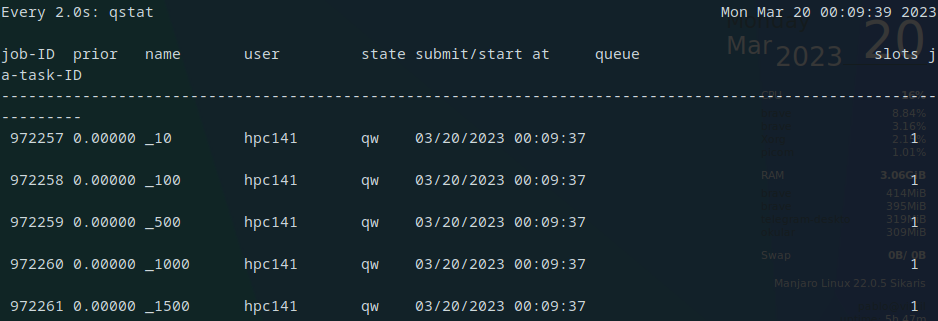
\includegraphics[width=0.5\textwidth]{watch.png}
\end{figure}

\newpage

\hypertarget{12}{%
\subsection{Provide a plot of the execution time of the application with the requested input
parameters. It is requested to include the average and standard deviation (or the
percentiles/quartiles of your choice) of various (e.g., 5-10) executions.}\label{12}}

At this point, a Python script was made to treat the results and to plot a box diagram. This script has two dependencies:
\begin{itemize}
    \item Pandas: a software library written for the Python programming language for data manipulation and analysis
    \item matplotlib: a comprehensive library for creating static, animated, and interactive visualizations in Python
\end{itemize}
\begin{lstlisting}[language=python, caption=Python program to treat data results]
import pandas as pd

from matplotlib import pyplot as plt
from os import walk

data = {}
# get data from results files
for dirpath, dirnames, filenames in walk("."):
    for filename in filenames:
        if filename.endswith(".txt"):
            key = int(filename.split(".")[0])
            with open(filename, "r") as _file:
                data[key] = [float(i) for i in _file.readlines()]

df = pd.DataFrame(data)
df = df.reindex(sorted(data.keys()), axis=1)

p = df.plot.box()
p.set_title("Sample parametric study")
p.set_xlabel("app parameter")
p.set_ylabel("Time (seconds)")
plt.show()
\end{lstlisting}
\textit{*For this exercise all results were placed in common files at same location of next script}.

This script loads all data from given txt files and build a Pandas DataFrame object. After this point, we need to reoder the indexes to have them in ascending order, label axis and give it a title to get our plot.

Below some tables show what information Pandas was able to retrieve with the provided data from result files:

\begin{table}
\centering
\begin{tabular}{|c|c|c|c|c|c|}
\hline
\textbf{Execution \ Input} & \textbf{10} & \textbf{100} & \textbf{500} & \textbf{1000} & \textbf{1500} \\ \hline
\textbf{1}                 & 0.05        & 0.85         & 3.26         & 14.57         & 22.15         \\ \hline
\textbf{2}                 & 0.00        & 0.30         & 1.45         & 13.48         & 29.00         \\ \hline
\textbf{3}                 & 0.06        & 0.66         & 3.30         & 11.55         & 22.28         \\ \hline
\textbf{4}                 & 0.01        & 0.01         & 0.90         & 12.76         & 17.60         \\ \hline
\textbf{5}                 & 0.01        & 0.31         & 4.49         & 9.99          & 20.89         \\ \hline
\textbf{6}                 & 0.05        & 0.25         & 5.42         & 11.37         & 24.88         \\ \hline
\textbf{7}                 & 0.04        & 0.74         & 3.86         & 8.01          & 28.62         \\ \hline
\textbf{8}                 & 0.02        & 0.22         & 5.27         & 6.27          & 24.13         \\ \hline
\textbf{9}                 & 0.05        & 0.65         & 5.08         & 5.45          & 20.51         \\ \hline
\textbf{10}                & 0.04        & 0.24         & 1.82         & 6.42          & 21.79         \\ \hline
\end{tabular}
\caption{\label{exec}Values of time command for each execution and input parameter.}
\vspace{2cm}
\begin{tabular}{|c|c|c|c|c|c|}
\hline
               & \textbf{10} & \textbf{100} & \textbf{500} & \textbf{1000} & \textbf{1500} \\ \hline
\textbf{count} & 10          & 10           & 10           & 10            & 10            \\ \hline
\textbf{mean}  & 0.033000    & 0.423000     & 3.485000     & 9.98700       & 23.185000     \\ \hline
\textbf{std}   & 0.021108    & 0.277611     & 1.643359     & 3.27079       & 3.567923      \\ \hline
\textbf{min}   & 0.000000    & 0.010000     & 0.900000     & 5.45000       & 17.600000     \\ \hline
\textbf{25\%}   & 0.012500    & 0.242500     & 2.180000     & 6.81750       & 21.115000     \\ \hline
\textbf{50\%}   & 0.040000    & 0.305000     & 3.580000     & 10.68000      & 22.215000     \\ \hline
\textbf{75\%}   & 0.050000    & 0.657500     & 4.932500     & 12.45750      & 24.692500     \\ \hline
\textbf{max}   & 0.060000    & 0.850000     & 5.420000     & 14.57000      & 29.000000     \\ \hline
\end{tabular}
\caption{\label{df}Extracted data from Table \ref{exec}.}
\end{table}

\pagebreak
\begin{figure}[h]
\caption{Execution time of the application with the requested input parameters}
\centering
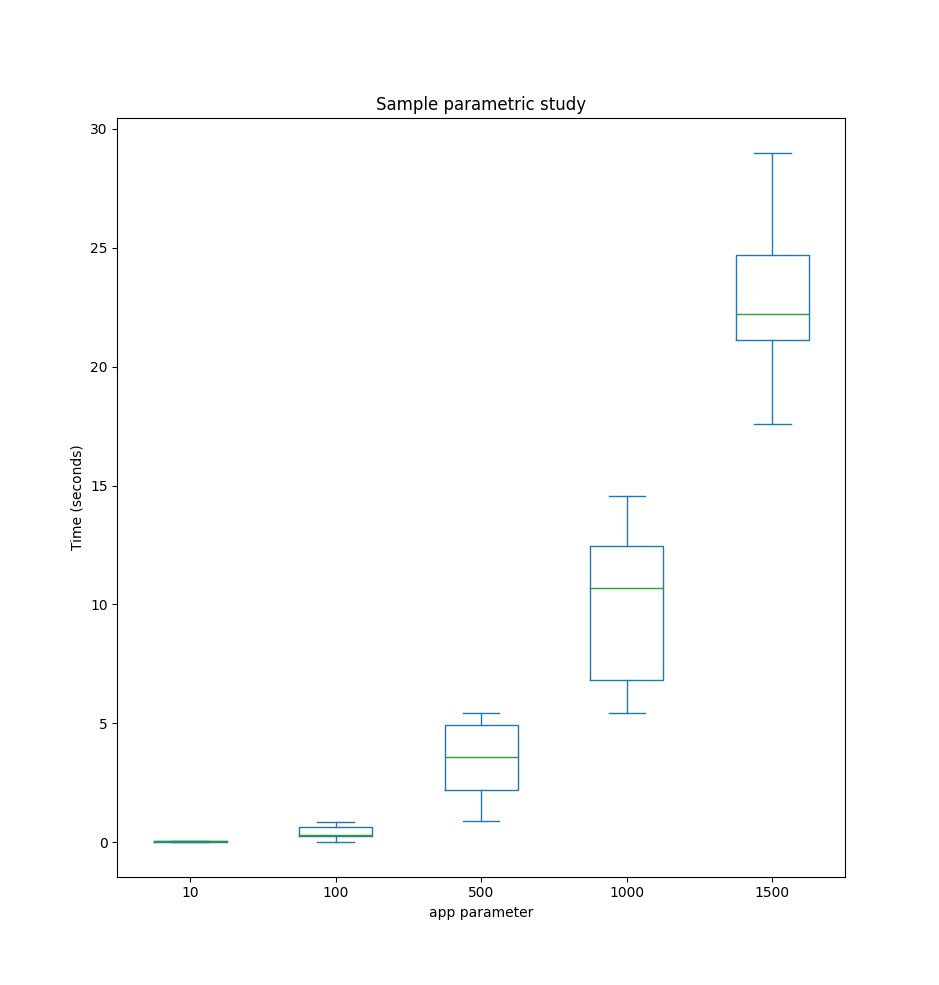
\includegraphics{boxes.png}
\end{figure}



\newpage

\hypertarget{2}{%
\section{Queuing System and Scheduling}\label{2}}

\hypertarget{FCFS}{%
\subsection{FCFS}\label{FCFS}}

In FCFS scheduling, the process that arrives first gets executed first, and so on. The CPU is allocated to the first process in the ready queue, and it continues to execute that process until it is either completed or blocked.

\begin{table}[]
\centering
\begin{tabular}{|c|c|c|c|c|c|c|c|c|c|c|c|}
\hline
\textbf{CPU\textbackslash{}Time} & \textbf{1} & \textbf{2} & \textbf{3} & \textbf{4} & \textbf{5} & \textbf{6} & \textbf{7} & \textbf{8} & \textbf{9}     & \textbf{10} & \textbf{11} \\ \hline
\textbf{CPU 1}                   & Job 1      & Job 1      & Job 1      & Job 1      & Job 1      & Job 1      & Job 1      & Job 1      & Job 4          & Job 4       & Job 4       \\ \hline
\textbf{CPU 2}                   & Job 1      & Job 1      & Job 1      & Job 1      & Job 1      & Job 1      & Job 1      & Job 1      & Job 4 & Job 4       & Job 4       \\ \hline
\textbf{CPU 3}                   & Job 1      & Job 1      & Job 1      & Job 1      & Job 1      & Job 1      & Job 1      & Job 1      & Job 4          & Job 4       & Job 4       \\ \hline
\textbf{CPU 4}                   & Job 1      & Job 1      & Job 1      & Job 1      & Job 1      & Job 1      & Job 1      & Job 1      & Job 4          & Job 4       & Job 4       \\ \hline
\textbf{CPU 5}                   & Job 1      & Job 1      & Job 1      & Job 1      & Job 1      & Job 1      & Job 1      & Job 1      & Job 5          & Job 5       &             \\ \hline
\textbf{CPU 6}                   & Job 1      & Job 1      & Job 1      & Job 1      & Job 1      & Job 1      & Job 1      & Job 1      &                &             &             \\ \hline
\textbf{CPU 7}                   & Job 1      & Job 1      & Job 1      & Job 1      & Job 1      & Job 1      & Job 1      & Job 1      &                &             &             \\ \hline
\textbf{CPU 8}                   & Job 1      & Job 1      & Job 1      & Job 1      & Job 1      & Job 1      & Job 1      & Job 1      &                &             &             \\ \hline
\textbf{CPU 9}                   &            & Job 2      & Job 2      & Job 3      & Job 3      & Job 3      & Job 3      & Job 3      & Job 3          & Job 3       & Job 3       \\ \hline
\textbf{CPU 10}                  &            & Job 2      & Job 2      &            &            &            &            &            &                &             &             \\ \hline
\end{tabular}
\caption{\label{FCFS1}FCFS from time slot 1 to 11}
\vspace{1cm}
\begin{tabular}{|c|c|c|c|c|c|c|c|c|c|c|}
\hline
\textbf{CPU\textbackslash{}Time} & \textbf{12} & \textbf{13} & \textbf{14} & \textbf{15} & \textbf{16} & \textbf{17} & \textbf{18} & \textbf{19} & \textbf{20} & \textbf{21} \\ \hline
\textbf{CPU 1}                   & Job 4       & Job 6       & Job 6       & Job 6       & Job 8       & Job 8       & Job 8       & Job 8       & Job 8       & Job 8       \\ \hline
\textbf{CPU 2}                   & Job 4       & Job 6       & Job 6       & Job 6       & Job 8       & Job 8       & Job 8       & Job 8       & Job 8       & Job 8       \\ \hline
\textbf{CPU 3}                   & Job 4       & Job 6       & Job 6       & Job 6       & Job 8       & Job 8       & Job 8       & Job 8       & Job 8       & Job 8       \\ \hline
\textbf{CPU 4}                   & Job 4       & Job 6       & Job 6       & Job 6       & Job 8       & Job 8       & Job 8       & Job 8       & Job 8       & Job 8       \\ \hline
\textbf{CPU 5}                   &             & Job 6       & Job 6       & Job 6       & Job 9       & Job 9       & Job 9       & Job 9       &             &             \\ \hline
\textbf{CPU 6}                   &             & Job 6       & Job 6       & Job 6       & Job 9       & Job 9       & Job 9       & Job 9       &             &             \\ \hline
\textbf{CPU 7}                   &             & Job 6       & Job 6       & Job 6       & Job 9       & Job 9       & Job 9       & Job 9       &             &             \\ \hline
\textbf{CPU 8}                   &             & Job 6       & Job 6       & Job 6       & Job 9       & Job 9       & Job 9       & Job 9       &             &             \\ \hline
\textbf{CPU 9}                   &             & Job 6       & Job 6       & Job 6       &             &             &             &             &             &             \\ \hline
\textbf{CPU 10}                  &             & Job 7       & Job 7       & Job 7       & Job 7       &             &             &             &             &             \\ \hline
\end{tabular}
\caption{\label{FCFS12}FCFS from time slot 12 to 21}
\vspace{1cm}
\begin{tabular}{|c|c|c|c|c|c|c|c|c|c|}
\hline
\textbf{CPU\textbackslash{}Time} & \textbf{22} & \textbf{23} & \textbf{24} & \textbf{25} & \textbf{26} & \textbf{27} & \textbf{28} & \textbf{29} & \textbf{30} \\ \hline
\textbf{CPU 1}                   & Job 10      & Job 10      & Job 11      & Job 11      & Job 11      & Job 11      &             &             & Job 16      \\ \hline
\textbf{CPU 2}                   & Job 10      & Job 10      & Job 11      & Job 11      & Job 11      & Job 11      &             &             & Job 16      \\ \hline
\textbf{CPU 3}                   & Job 10      & Job 10      & Job 12      & Job 12      & Job 12      & Job 12      &             &             & Job 16      \\ \hline
\textbf{CPU 4}                   & Job 10      & Job 10      & Job 12      & Job 12      & Job 12      & Job 12      &             &             & Job 16      \\ \hline
\textbf{CPU 5}                   & Job 10      & Job 10      & Job 13      & Job 13      & Job 13      & Job 13      &             &             & Job 16      \\ \hline
\textbf{CPU 6}                   & Job 10      & Job 10      & Job 14      & Job 14      & Job 14      & Job 14      &             &             &             \\ \hline
\textbf{CPU 7}                   & Job 10      & Job 10      & Job 15      & Job 15      & Job 15      & Job 15      & Job 15      & Job 15      &             \\ \hline
\textbf{CPU 8}                   & Job 10      & Job 10      &             &             &             &             &             &             &             \\ \hline
\textbf{CPU 9}                   & Job 10      & Job 10      &             &             &             &             &             &             &             \\ \hline
\textbf{CPU 10}                  & Job 10      & Job 10      &             &             &             &             &             &             &             \\ \hline
\end{tabular}
\caption{\label{FCFS22}FCFS from time slot 22 to 30}
\end{table}

\begin{table}
\centering
\begin{tabular}{|c|c|c|c|c|c|}
\hline
\textbf{CPU\textbackslash{}Time} & \textbf{31} & \textbf{32} & \textbf{33} & \textbf{34} & \textbf{35} \\ \hline
\textbf{CPU 1}                   & Job 16      & Job 17      & Job 17      & Job 17      & Job 18      \\ \hline
\textbf{CPU 2}                   & Job 16      & Job 17      & Job 17      & Job 17      & Job 18      \\ \hline
\textbf{CPU 3}                   & Job 16      & Job 17      & Job 17      & Job 17      & Job 18      \\ \hline
\textbf{CPU 4}                   & Job 16      & Job 17      & Job 17      & Job 17      &             \\ \hline
\textbf{CPU 5}                   & Job 16      & Job 17      & Job 17      & Job 17      &             \\ \hline
\textbf{CPU 6}                   &             & Job 17      & Job 17      & Job 17      &             \\ \hline
\textbf{CPU 7}                   &             & Job 17      & Job 17      & Job 17      &             \\ \hline
\textbf{CPU 8}                   &             & Job 17      & Job 17      & Job 17      &             \\ \hline
\textbf{CPU 9}                   &             & Job 17      & Job 17      & Job 17      &             \\ \hline
\textbf{CPU 10}                  &             &             &             &             &             \\ \hline
\end{tabular}
\caption{\label{FCFS31}FCFS from time slot 31 to 35}
\end{table}

\begin{center}
Utilization = Used slots / Total slots = $\frac{255}{350} = \textbf{72.85\%}$
\end{center}

\newpage

\hypertarget{EASY-backfilling}{%
\subsection{EASY-backfilling}\label{EASY-backfilling}}

 In EASY-backfilling, the scheduler first applies the FCFS policy to the incoming processes. If a new job arrives while an existing job is being executed, and if the new job can be scheduled to complete before the existing job finishes, the new job is backfilled in the remaining time of the existing job.

This approach helps to minimize the wait time of short processes by allowing them to get executed ahead of long processes that arrived earlier, and also maximizes the utilization of the CPU by filling up the remaining time of longer processes with shorter processes.

\begin{table}[]
\centering
\begin{tabular}{|c|c|c|c|c|c|c|c|c|c|c|c|}
\hline
\textbf{CPU\textbackslash{}Time} & \textbf{1} & \textbf{2} & \textbf{3} & \textbf{4} & \textbf{5} & \textbf{6} & \textbf{7} & \textbf{8} & \textbf{9}     & \textbf{10} & \textbf{11} \\ \hline
\textbf{CPU 1}                   & Job 1      & Job 1      & Job 1      & Job 1      & Job 1      & Job 1      & Job 1      & Job 1      & Job 4          & Job 4       & Job 4       \\ \hline
\textbf{CPU 2}                   & Job 1      & Job 1      & Job 1      & Job 1      & Job 1      & Job 1      & Job 1      & Job 1      & \textbf{Job 4} & Job 4       & Job 4       \\ \hline
\textbf{CPU 3}                   & Job 1      & Job 1      & Job 1      & Job 1      & Job 1      & Job 1      & Job 1      & Job 1      & Job 4          & Job 4       & Job 4       \\ \hline
\textbf{CPU 4}                   & Job 1      & Job 1      & Job 1      & Job 1      & Job 1      & Job 1      & Job 1      & Job 1      & Job 4          & Job 4       & Job 4       \\ \hline
\textbf{CPU 5}                   & Job 1      & Job 1      & Job 1      & Job 1      & Job 1      & Job 1      & Job 1      & Job 1      & Job 7          & Job 7       & Job 7       \\ \hline
\textbf{CPU 6}                   & Job 1      & Job 1      & Job 1      & Job 1      & Job 1      & Job 1      & Job 1      & Job 1      &                &             &             \\ \hline
\textbf{CPU 7}                   & Job 1      & Job 1      & Job 1      & Job 1      & Job 1      & Job 1      & Job 1      & Job 1      &                &             &             \\ \hline
\textbf{CPU 8}                   & Job 1      & Job 1      & Job 1      & Job 1      & Job 1      & Job 1      & Job 1      & Job 1      &                &             &             \\ \hline
\textbf{CPU 9}                   &            & Job 2      & Job 2      & Job 3      & Job 3      & Job 3      & Job 3      & Job 3      & Job 3          & Job 3       & Job 3       \\ \hline
\textbf{CPU 10}                  &            & Job 2      & Job 2      &            &            & Job 5      & Job 5      &            &                &             &             \\ \hline
\end{tabular}
\caption{\label{EASY1}EASY-backfilling from time slot 1 to 11}
\vspace{1cm}
\begin{tabular}{|c|c|c|c|c|c|c|c|c|c|c|}
\hline
\textbf{CPU\textbackslash{}Time} & \textbf{12} & \textbf{13} & \textbf{14} & \textbf{15} & \textbf{16} & \textbf{17} & \textbf{18} & \textbf{19} & \textbf{20} & \textbf{21} \\ \hline
\textbf{CPU 1}                   & Job 4       & Job 6       & Job 6       & Job 6       & Job 8       & Job 8       & Job 8       & Job 8       & Job 8       & Job 8       \\ \hline
\textbf{CPU 2}                   & Job 4       & Job 6       & Job 6       & Job 6       & Job 8       & Job 8       & Job 8       & Job 8       & Job 8       & Job 8       \\ \hline
\textbf{CPU 3}                   & Job 4       & Job 6       & Job 6       & Job 6       & Job 8       & Job 8       & Job 8       & Job 8       & Job 8       & Job 8       \\ \hline
\textbf{CPU 4}                   & Job 4       & Job 6       & Job 6       & Job 6       & Job 8       & Job 8       & Job 8       & Job 8       & Job 8       & Job 8       \\ \hline
\textbf{CPU 5}                   & Job 7       & Job 6       & Job 6       & Job 6       & Job 9       & Job 9       & Job 9       & Job 9       & Job 16      & Job 16      \\ \hline
\textbf{CPU 6}                   &             & Job 6       & Job 6       & Job 6       & Job 9       & Job 9       & Job 9       & Job 9       & Job 16      & Job 16      \\ \hline
\textbf{CPU 7}                   &             & Job 6       & Job 6       & Job 6       & Job 9       & Job 9       & Job 9       & Job 9       & Job 16      & Job 16      \\ \hline
\textbf{CPU 8}                   &             & Job 6       & Job 6       & Job 6       & Job 9       & Job 9       & Job 9       & Job 9       & Job 16      & Job 16      \\ \hline
\textbf{CPU 9}                   &             & Job 6       & Job 6       & Job 6       &             &             &             &             & Job 16      & Job 16      \\ \hline
\textbf{CPU 10}                  &             &             &             &             &             &             &             &             &             &             \\ \hline
\end{tabular}
\caption{\label{EASY12}EASY-backfilling from time slot 12 to 21}
\vspace{1cm}
\begin{tabular}{|c|c|c|c|c|c|c|}
\hline
\textbf{CPU\textbackslash{}Time} & \textbf{22} & \textbf{23} & \textbf{24} & \textbf{25} & \textbf{26} & \textbf{27} \\ \hline
\textbf{CPU 1}                   & Job 10      & Job 10      & Job 11      & Job 11      & Job 11      & Job 11      \\ \hline
\textbf{CPU 2}                   & Job 10      & Job 10      & Job 11      & Job 11      & Job 11      & Job 11      \\ \hline
\textbf{CPU 3}                   & Job 10      & Job 10      & Job 12      & Job 12      & Job 12      & Job 12      \\ \hline
\textbf{CPU 4}                   & Job 10      & Job 10      & Job 12      & Job 12      & Job 12      & Job 12      \\ \hline
\textbf{CPU 5}                   & Job 10      & Job 10      & Job 13      & Job 13      & Job 13      & Job 13      \\ \hline
\textbf{CPU 6}                   & Job 10      & Job 10      & Job 14      & Job 14      & Job 14      & Job 14      \\ \hline
\textbf{CPU 7}                   & Job 10      & Job 10      & Job 15      & Job 15      & Job 15      & Job 15      \\ \hline
\textbf{CPU 8}                   & Job 10      & Job 10      & Job 18      &             &             &             \\ \hline
\textbf{CPU 9}                   & Job 10      & Job 10      & Job 18      &             &             &             \\ \hline
\textbf{CPU 10}                  & Job 10      & Job 10      & Job 18      &             &             &             \\ \hline
\end{tabular}
\caption{\label{EASY22}EASY-backfilling from time slot 22 to 27}
\end{table}

\begin{table}
\centering
\begin{tabular}{|c|c|c|c|c|c|}
\hline
\textbf{CPU\textbackslash{}Time} & \textbf{28} & \textbf{29} & \textbf{30} & \textbf{31} & \textbf{32} \\ \hline
\textbf{CPU 1}                   &             &             & Job 17      & Job 17      & Job 17      \\ \hline
\textbf{CPU 2}                   &             &             & Job 17      & Job 17      & Job 17      \\ \hline
\textbf{CPU 3}                   &             &             & Job 17      & Job 17      & Job 17      \\ \hline
\textbf{CPU 4}                   &             &             & Job 17      & Job 17      & Job 17      \\ \hline
\textbf{CPU 5}                   &             &             & Job 17      & Job 17      & Job 17      \\ \hline
\textbf{CPU 6}                   &             &             & Job 17      & Job 17      & Job 17      \\ \hline
\textbf{CPU 7}                   & Job 15      & Job 15      & Job 17      & Job 17      & Job 17      \\ \hline
\textbf{CPU 8}                   &             &             & Job 17      & Job 17      & Job 17      \\ \hline
\textbf{CPU 9}                   &             &             &             &             &             \\ \hline
\textbf{CPU 10}                  &             &             &             &             &             \\ \hline
\end{tabular}
\caption{\label{EASY28}EASY-backfilling from time slot 28 to 32}
\end{table}

\begin{center}
Utilization = Used Slots / Total Slots = $\frac{252}{320} = \textbf{78.75\%}$
\end{center}

\newpage

\appendix

\section{Data Files}
\subsection{10.txt}
\lstinputlisting{10.txt}
\subsection{100.txt}
\lstinputlisting{100.txt}
\subsection{500.txt}
\lstinputlisting{500.txt}
\subsection{1000.txt}
\lstinputlisting{1000.txt}
\subsection{1500.txt}
\lstinputlisting{1500.txt}

\section{SGE files}
\subsection{10.sge}
\lstinputlisting[language=bash]{10.sge}
\subsection{100.sge}
\lstinputlisting[language=bash]{100.sge}
\subsection{500.sge}
\lstinputlisting[language=bash]{500.sge}
\subsection{1000.sge}
\lstinputlisting[language=bash]{1000.sge}
\subsection{1500.sge}
\lstinputlisting[language=bash]{1500.sge}

\section{Scripts}
\subsection{run.sh}
\lstinputlisting[language=bash]{run.sh}
\subsection{plot.py}
\lstinputlisting[language=python, caption]{plot.py}

\end{document}

